\section{Tepelný management}
-význam pro pouzdření, způsoby šíření tepla, náhradní tepelný obvod pouzdra s tranzistorem, analogie mezi elektrickými a tepelnými veličinami

\subsection{Význam pro pouzdření}
Kovová nebo keramická pouzdra budou odvádět lépe teplo, než např. plastová


\subsection{Šíření tepla}
\begin{itemize}
\item vedením (kundukce)
\item prouděním (konvekce)
\item zářením (radiace)
\end{itemize}
Tyto tři způsoby šíření tepla se dějí současně.

\textbf{Vedení (kondukce) tepla} je jeden ze způsobů šíření tepla v tělesech, při kterém částice látky v oblasti s vyšší střední kinetickou energií předávají část své pohybové energie prostřednictvím vzájemných srážek částicím v oblasti s nižší střední kinetickou energií. Částice se přitom nepřemísťují, ale kmitají kolem svých rovnovážných poloh.

Vedení tepla je způsob šíření tepla v pevných tělesech, jejichž různé části mají různé teploty. Teplo se vedením šíří také v kapalinách a plynech, kde se však uplatňuje také šíření tepla prouděním.

\textbf{Šíření tepla prouděním (konvekcí)} je jeden ze způsobů šíření tepla, kdy dochází k proudění hmoty o různé teplotě. Šíření tepla prouděním není možné u pevných látek, uplatňuje se pouze u tekutin (kapalin a plynů), případně u plazmatu. Pohybem hmoty dochází k vzájemnému pohybu jednotlivých částí, které mají odlišnou teplotu a tedy různou hustotu vnitřní energie, a tím se přenáší teplo.

\textbf{Záření (vyzařování, radiace)} je fyzikální proces, při kterém látka emituje do prostoru energii ve formě elektromagnetického záření. Na rozdíl od přenosu tepla vedením nebo prouděním se může prostřednictvím sálání teplo přenášet i ve vakuu, tzn. bez zprostředkování přenosu látkovým prostředím.
Energie, která je sáláním vyzařována, závisí na několika faktorech:
\begin{itemize}
\item teplota tělesa – množství vyzářené energie
\item barva povrchu – nejmenší množství tepla je vyzařováno stříbřitě lesklými povrchy, největší černými. Toho se využívá například při konstrukci termosek, kde jsou povrchy stříbřitě lesklé pro minimalizaci předávání tepla sáláním. Jiným příkladem jsou naopak chladiče kosmických lodí, které jsou černé pro maximalizaci vyzářeného tepla. Při teplotách nad 1000 $^{\circ}$C je ale pro většinu materiálů již rozdíl zanedbatelný a s malou chybou lze počítat s tím, že se prakticky všechna tělesa chovají jako absolutně černé těleso.
\item obsah plochy – energie vyzařovaná sáláním je přímo úměrná obsahu povrchu vyzařujícího tělesa.
\end{itemize}

\subsection{Náhradní tepelný obvod pouzdra s tranzistorem, analogie mezi elektrickými a tepelnými veličinami}

\begin{figure}[h]
   \begin{center}
     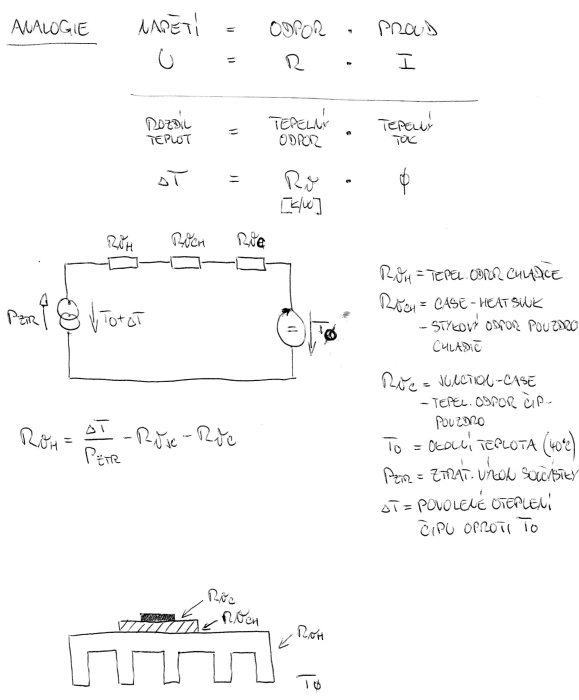
\includegraphics[scale=0.6]{images/Analogie.png}
   \end{center}
   \caption{Analogie}
\end{figure}